\documentclass[a4paper,11pt]{article}
\usepackage[T1]{fontenc}
\usepackage[ngerman]{babel}
\usepackage{graphicx}
\usepackage{listings}
\usepackage{color}

\definecolor{dkgreen}{rgb}{0,0.6,0}
\definecolor{gray}{rgb}{0.5,0.5,0.5}
\definecolor{mauve}{rgb}{0.58,0,0.82}

\lstset{frame=tb,
  language=Go,
  aboveskip=3mm,
  belowskip=3mm,
  showstringspaces=false,
  columns=flexible,
  basicstyle={\small\ttfamily},
  numbers=none,
  numberstyle=\tiny\color{gray},
  keywordstyle=\color{blue},
  commentstyle=\color{dkgreen},
  stringstyle=\color{mauve},
  breaklines=true,
  breakatwhitespace=true,
  tabsize=3
}

\title{
  Entwicklung eines Operator zur Installation und 
  \textit{2
  \textsuperscript{nd} day operations
  } von Sormasinstanzen auf Kubernetes.
}
\date{07.07.2020}
\author{Nico Kahlert}
\begin{document}
  \maketitle
  \newpage
  \tableofcontents
  \newpage
  \pagenumbering{arabic}
  \vspace{2.5cm}
  \section{Einleitung}
    \subsection{Vortellung des Kunden}
    Die Netzlink Informationstechnik GmbH ist ein IT-Systemhaus mit ca. 90
    Mitarbeitern. Zur Zielgruppe des Unternehmens gehören hauptsächlich 
    Kundes aus dem Mittelstand, für welche IT-Dienstleistungen On-Premise oder in der Cloud
    erbracht werden. Die drei Firmenstandorte befinden sich in Braunschweig, Kassel und Hannover.
    Außerdem führt Netzlink drei georedundante Rechenzentren in Hannover, Salzgitter und Braunschweig.
    Jene dienen sowohl der eigenen Infrastruktur, als auch Kundenprojekten. 
    \subsection{Auswahl des Projektes}
    Die bis zum Verfassungszeitpunkt andauernde Krise um die Pandemie des SARS-Cov-2 Erregers 
    in den Jahren 2019/2020, hat einen Bedarf an Software zur zentralen Dokumentation und Analyse 
    einer Epidemie ausgelöst. Um das Cloudportfolio der neuen Herausforderung anzupassen, wurde die Sormas-
    software ,in direkter Partnershaft mit dem Helmholtzzentrum für Infektionsforschung, als SAAS Lösung 
    aufgenommen. \newline >>///<<Hier erweitern>>///<<
      \subsubsection{Sormas}
      Sormas ist eine eine quelloffene Softwarelösung zum Management und der Analyse von Epidemien.
      Entwickler ist die Firma Symeda und das Helmholtzzentrum für Infektionsforschung Braunschweig.
      Der ursprüngliche Einsatzzweck von Sormas war die Eindämmung und das Management der 
      Ebolaepidemie in Westafrika im Jahr 2014, wo sie bis heute eingesetzt wird.
      \newline Die Lösung besteht im großenganzen aus vier Komponenten: Einem relationalen 
      Postgresdatenbankmanagementsystems in welchem der gesamte Datenstand gehalten wird. Einem 
      Optionalen Mailserver zum Verschicken von E-Mailbenachrichtigungen. Einem Hazelcast-LRU-Cache
      ,welcher in den Payara eingebettet oder extern betrieben werden kann und zur temporären Speicherung
      der Nutzersitzungen dient. Und zuletzt einem Javaapplikationsserver von Payara auf welchem Javaapplikationen 
      ausgeführt werden. Bei Sormas wurden zwei Javaservlet entwickelt, welche die Applikationslogik beinhalten.
      Das \textit{web-ui} Servlet stellt eine Javascript basierte, grafische Nutzerschnittstelle  über das Web 
      bereit an dem der Nutzer Plattformunabhängig arbeiten kann. Außerdem gibt es ein \textit{rest} Servlet, welches
      eine REST-API für die Apps mobiler Endgeräte bereitstellt. Zur Installation auf einem Host werden 
      Containerimages und dazugehörige Konfigurationsdateinen von Netzlink gebaut und auf Github angeboten.
      Sormas und seine Komponenten sind komplett quelloffene Software, so ist eine Transparenz gegenüber dem
      Kunden gewährleistet. Die Lizenzen der einzenen Projekte sind jedoch teilweise absent und somit proprietär.
      \subsubsection{Kubernetes}
      Seit einigen Jahren hat sich die Arbeitswelt der Informationstechnik stark verändert.
      Die großen Internetdienste wie Suchmaschienen, Wissensdatenbanken, Videoplattformen oder Sozialemedien wurden 
      in letztem Jahrzehnt zu unversichbarer Infrastruktur für Menschen auf der gesamten Welt. Ein Ausfall von Sekunden oder mehr 
      kostet diesen Unternehmen und Nutzern viel Geld. Software muss heutzutage Redundant abgesichert sein und per Failover Ausfälle vermeiden können.
      Aber Redundanz der Software heißt immer auch redundante Infrastruktur ,jedoch kostet Rechenzeit und Betrieb der Server viel Geld. Um dieser 
      Nachfrage standzuhalten braucht es eine Lösung, die sich nach den Bedürfnissen der Nutzer hochskalieren lässt, aber bei weniger Anfragen 
      automatisch weniger Infrastruktur benötigt. Eine weitere Entwicklung der Jahre zeigt der Verlauf der Leistung von CPUs.
      Nach \textit{mooreschem Gesetz} (Abbildung \ref{fig:moores_law}) werden ICs (integrierte Schaltkreise), wozu auch CPUs zählen, regelmäßig Komplexer,
      wobei sich auch die Schaltgeschwindigkeit erhöht und eine höhere Leistung generell erziehlt werden kann.
      \begin{figure}[!ht]
        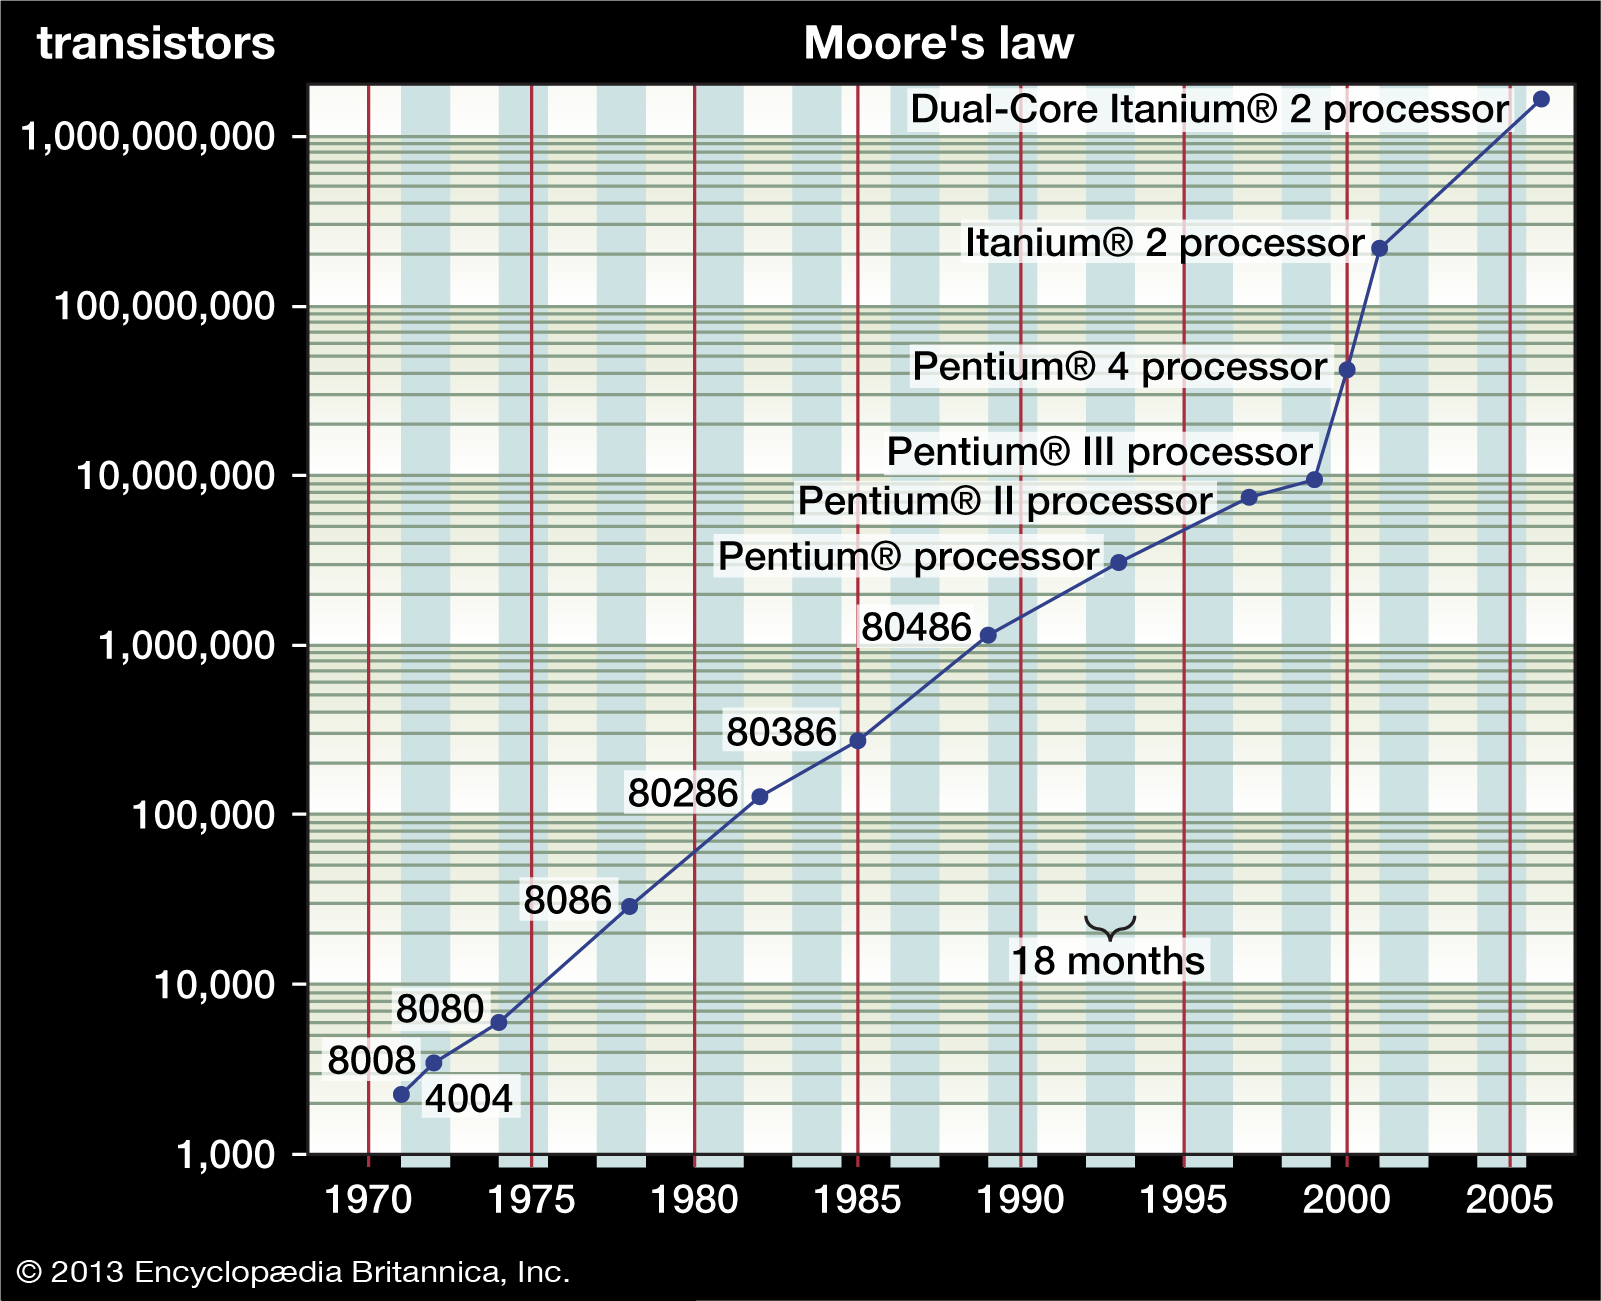
\includegraphics[width=0.6\linewidth]{assets/gordon-EeMoore-law-number-transistors-computer.jpg}
        \caption{Moorisches Gesetz}
        \label{fig:moores_law}
      \end{figure}
      Allerdings ist die Technik vom heutigen Stand an einem Punkt gekommen, an dem physikalische Grenzen eine regelmäßige Verkleinerung
      von den Transistoren erheblich erschwert. An diesem Punkt machen nun mehr unterschiedliche Prozessorarchitekturen in Einzelmaschienen einen 
      Unterschied. Da jedoch die meiste Software auf die vorherschende x86-Plattform angepasst ist das oft nicht möglich. Der bessere Ansatz ist 
      eine \textit{scale-out} Strategie, welche die Rechenzeit mehrerer Server für eine Aufgabe bündelt. Dies löst nicht nur das Problem der 
      fehlenden Leistung einzelner Maschinen sondern auch das Problem der Redundanz. Ein weiteres Problem der \emph{Big Player} in der Informationstechnik
      ist der riesige Maßstab Ihrer Umgebungen. Um Gesamtheit der Services auf gewünschtem Stand zu halten benötigt man eine Technologie, welche es erlaubt,
      eine Umgebung \emph{deklarativ} zu managen. Seit 2012 mit der popularisierung von Containern durch die Docker Inc. gibt es die Möglichkeit seine
      Dienste und die dazugehörige Umgebung, dazu gehören Softwarebibliotheken, Services und Konfigurationsdateinen, in ein sogenanntes Image zu
      verpacken und über das Netzwerk oder Internet zu verteilen. Das Interessante hier ist das es Container erlauben einen Dienst zu benutzen, ohne ihn 
      jemals installiert zu haben. Abbildung 2 zeigt noch einen Vorteil von Containern zu virtuellen Maschinen auf:\newline
      Virtuelle Maschinen beinhalten immer ein komplettes Betriebssystem, wobei Container den Kernel des \emph{Containerhosts} für Systemaufrufe nutzen.
      So lassen sich mehrere Services leichtgewichtig und nachhaltig nebeneinander betreiben, ohne bei Kompartimentiereung einbüßen zu müssen.  
      \begin{figure}[!ht]
        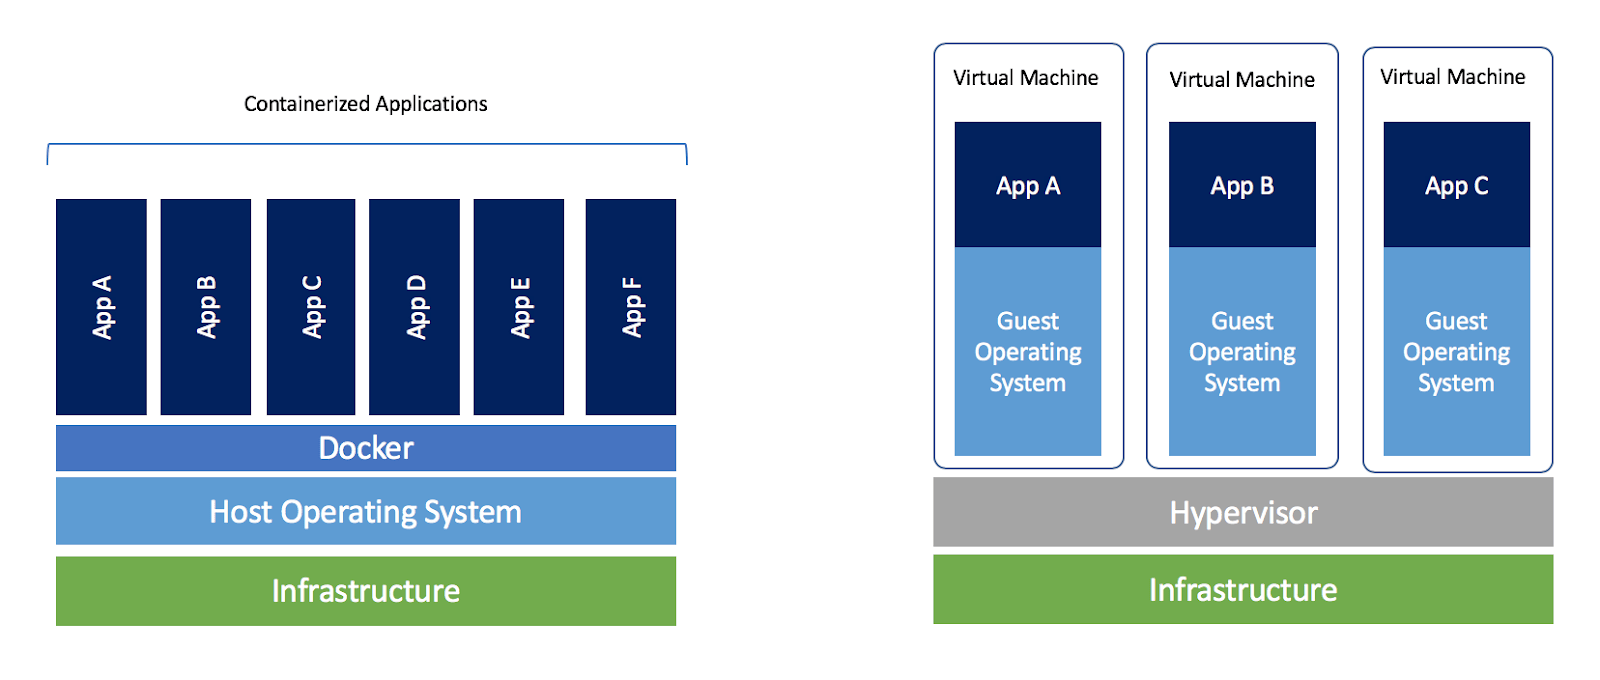
\includegraphics[width=\linewidth]{assets/containers-vm.jpg}
        \caption{Container/VM Gegenüberstellung}
        \label{fig:container_vm}
      \end{figure}
      Google Inc. und andere IT-Firmen aus dem Silicon Valley haben sich den oben genannten Problemen gestellt und
      eine Plattform entwickelt, die diese Branche von Grund auf verändert hat: Die seit 2014 quelloffene 
      Containerplattform namens Kubernetes (griechisch für Segler). Die PLattform besteht aus mehreren Comptern, denen unterschiedliche
      Rollen zugewiesen sind. Abbildung \ref{fig:kubernetes_arch} gibt einen Überblick der Services die ein Kubernetes ausmachen.
      Master haben die Aufgabe die API des Clusters bereitzustellen und die Arbeitslast auf verschiedene (Worker)-Nodes zu verteilen, was vom 
      \emph{kube-scheduler erledigt wird}. Die Aufgabe des \emph{kube-controller manager} ist der continuierliche Vergleich von \emph{Ist}- und 
      \emph{Sollzustand} der Konfiguration, wobei Unterschiede zum \emph{Sollzustand} angepasst werden. Die Konfiguration des Clusters ist 
      global in einem verteiltem \emph{Key-Value-Store}, dem \emph{ETCD}. Diese Datenbank bildet ebenfalls ein Cluster und ist nach dem CAP-Theorem
      als eine konsistente und partitionstolerante Datenbank einzuordnen. Quorum wird hier durch den Konsenzalgorithmus \emph{Raft} gebildet.
      Die zweite Gruppe der Hosts sind die \emph{Worker}, auf welchen der \emph{Kubelet}-service Container mittels einer OCI-kompatiblen Containerruntime
      betreibt.
      \begin{figure}[!ht]
        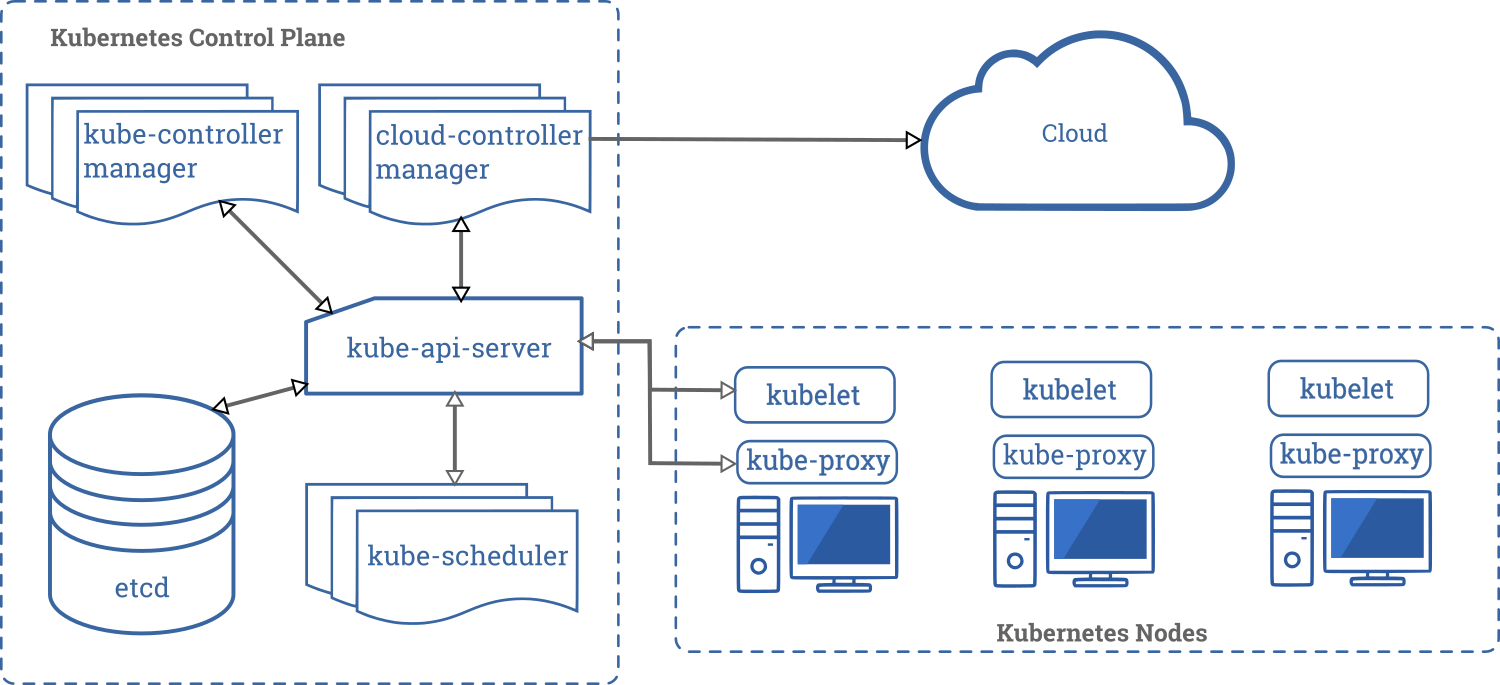
\includegraphics[width=\linewidth]{assets/components-of-kubernetes.png}
        \caption{Architektur von Kubernetes}
        \label{fig:kubernetes_arch}
      \end{figure}
      Die Konfigurationsdateien sind in JSON oder YAML geschrieben und werden vom User an die REST-API des Clusters geschickt. Durch die deklarative Natur des Systems
      werden die deklarierten Services auf den Workern aufgebaut.
      \subsubsection{RedHat OpenShift Container Plattform}
      Die OpenShift Container Plattform ist eine \textit{enterprisegrade} Kubernetesdistribution der Firma RedHat. Neben den
      Funktionalitäten von Kubernetes beinhaltet die Plattform einen Supportvertrag und Verbesserungen im Bereich 
      Lifecyclemanagement und Administrationsaufwand auf Kosten der Leichtgewichtigkeit (Abbildung \ref{fig:openshift_arch}).
      \begin{figure}[!ht]
        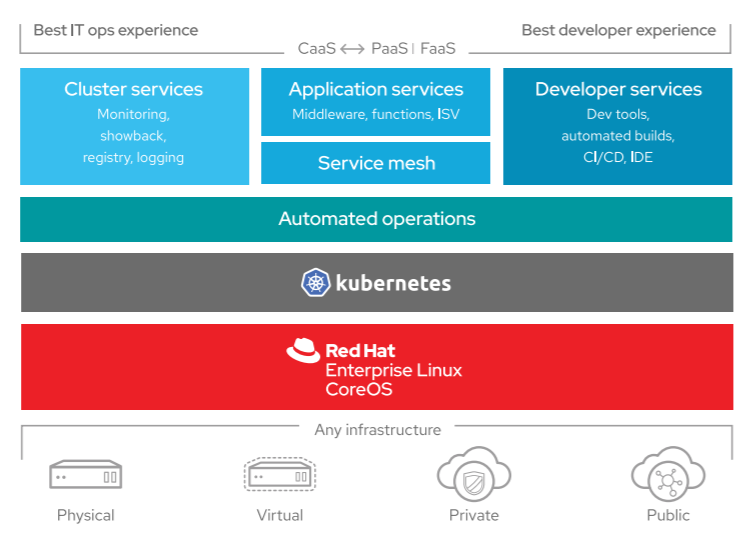
\includegraphics[width=\linewidth]{assets/openshift.png}
        \caption{Architektur von OpenShift}
        \label{fig:openshift_arch}
      \end{figure}
      \subsubsection{Golang}
      Golang ist eine junge, multiparadigmatische Programmiersprache der C-Familie. Sie ist eine kompilierte Sprache und produziert ausführbaren
      Maschinencode für alle verbreiteten Prozessorarchitekturen. Entwickelt wurde \emph{Go} unter anderem von dem Turingawardpreisträger, Unixentwickler und 
      Computerpionier Ken Thompson bei Google, als verständlicherer Ersatz für die Programmiersprache C++. Das Maskottchen der Programmiersprache ist der Gopher,
      bekannt aus dem Betriebssystem Plan 9 der Bell Labs (Abbildung \ref{fig:gopher}).
      \begin{figure}[!ht]
        
\includegraphics[width=0.3\linewidth]{assets/gopher.png}
        \caption{Golang Maskottchen: Der Gopher}
        \label{fig:gopher}
      \end{figure}
      Wie C++ ist Go auch Objektorientiert, wobei die Objektorientierung
      auf dem starken Typensystem von Go aufbaut. Anstatt von Vererbung wird in Go \emph{composition} angewendet, wobei ein Typ einen anderen Typen beinhaltet und somit ein 
      neuer Typ auf basis der Ersteren entsteht. Eine Besonderheit der Sprache ist die Möglichkeit in der Definition von Typen Annotationen anzugeben, die bei der
      überführung des Objektes in eine Datenbeschreibungssprache wie JSON, YAML oder Protobufer helfen.
      \begin{lstlisting}
          type Sormas struct {
            	metav1.TypeMeta         `json:",inline"`
            	metav1.ObjectMeta       `json:"metadata,omitempty"`

              	Spec   SormasSpec       `json:"spec,omitempty"`
              	Status SormasStatus     `json:"status,omitempty"`
          }
      \end{lstlisting}
      \emph{Beispielcode für einen Typen in Golang mit Annotation für JSON}\newline
      In diesem Projekt habe ich mich für die Programmiersprache Go entschieden, da gewisse Kenntnisse im OpenSolutions Team vorherschen und Kubernetes selbst in Go verfasst ist.
      Das ist ein großer Vorteil, da einfach bestehende Programmteile aus den Repositorys von Kubernetes übernommen werden können.
      \subsubsection{Operator Framework}
      Kubernetes bietet mit seinen nativen Objekten einen guten Grund um die eigenen Services 
      abbilden zu können. Anstatt selbst Container auf Hosts zu starten wird dies vom Orchestrator erledigt.
      Doch gibt es Aufgaben die so speziell an einen Service gebunden sind, das der Mensch eingreifen muss.
      Dazu zählen administrative Aufgaben wie das sichere Updaten einer Applikation oder die Migration von Umgebungen,
      aber auch das Erstellen von Nutzern und die gesamten 2\textsuperscript{nd} Day Operations.
      Um diese Aufgaben zu Automatisieren, kann das Modell eines \emph{Controllers} nach Kubernetes in Kombination einer 
      \emph{Custom Resource Definition} benutzt werden. Dieses Vorgehen beschreibt das von 
      RedHat geprägte \emph{Operatorpattern}. Eine \emph{Custom Resource Definition} beschreibt ein eigens hinzugefügtes
      Objekt als Erweiterung der Kubernetes-API. Es folgt dem Aufbau anderer Kubernetesobjekte und ist einer \emph{API-Group}, sowie einem \emph{Kind} zugewiesen.
      Dieses \emph{Custom Resource Definition} beinhaltet außerdem eine Beschreibung der Konfigurationsmöglichkeiten des Objekts.
      Ein \emph{Controller} ist eine Software, die eine oder mehrere Objekte der Kubernetes-API beobachtet und Änderungen durchsetzt.
      Dieser unaufhörliche Vergleich wird \emph{reconcile loop} genannt, also eine Vereinung von theoretischer Konfiguration und dem echtem Zustand (Abbildung \ref{fig:reconcile_loop}). 
      \begin{figure}[!ht]
        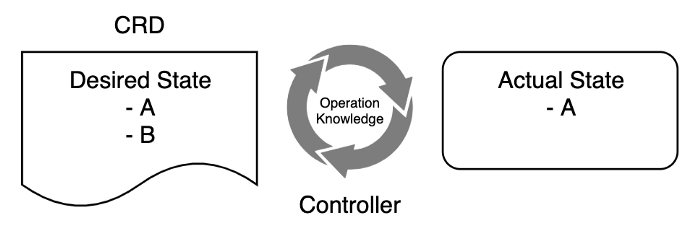
\includegraphics[width=\linewidth]{assets/operator_loop.png}
        \caption{Funktion eines Operators}
        \label{fig:reconcile_loop}
      \end{figure}
      Theoretisch ist es möglich einen Operator in jeder Programmiersprache mit Netzwerkimplementation zu schreiben (z.B. Bash, Lisp, Powershell), jedoch
      hat RedHat ein Framework und zugehöriges Entwicklungswergzeug für die Programmiersprache Golang entwickelt und der Gemeinschaft überlassen.
      Somit kann jeder Programmierer einigermaßen Kubernetes- und Golangerfahrung einen Operator in kurzer Zeit entwickeln, ohne von Grund auf anzufangen.
      Aus diesem Grund benutze Ich in diesem Projekt das OperatorSDK. Einen Zusatz den dieses mit sich bringt ist die Integration der Objekte in die 
      grafische Weboberfläche des Clusters, was in diesem Projekt nicht weiter beachtet wird.
    \subsection{Wirtschaftliche Betrachtung}
    Da Netzlink ein bestehendes OpenShift Cluster in seinem Rechenzentrum in Braunschweig betreibt, fallen für die Entwicklung und den Betrieb keine Kosten an,
    die Kosten des Projekts beziehen sich Ausschließlich auf meinen Verbleib aus dem Tagesgeschäft. Also ergibt sich folgende Tabelle:
    \begin{table}[!ht]
        \centering
        \caption{Wirtschaftliche Betrachtung}
        \label{tab:wirt-betr}
        \begin{tabular}{lllll}
         Aufgabe &  Aufwand (h) & Kosten (EUR)  \\
         Evaluierung des Objekttyps der Komponenten & 0.5 & 30  \\
         Schreiben der Manifeste & 3.5 & 210 \\
         Initialisierung des Projektes & 0.5 & 30 \\
         Beschreibung der API-Objekte und Typen & 2 & 120 \\
         Beschreibung der Reconcile-logic & 8 &  480 \\
         Anwenden der Reconcielogic & 10.5 & 630 \\
         Installation des Operators und einer Instanz & 0.5 & 30 \\
         Test der Instanz & 0.5 & 30 \\
         Durchführung eines Updates der Instanz & 0.5 & 30 \\
         Überprüfung der Updates & 0.5 & 30 \\
         Anfertigung der Dokumentation & 8 & 480 \\
         Gesamt & 35  & 2100 \\
        \end{tabular}
    \end{table}
    \subsection{Nachhaltige Betrachtung} 
    Da Sormas zur Zeit auf virtuellen Maschinen ausgerollt wird, ist es auch interessant,
    sich die verbrauchten Ressourcen anzuschauen:
    \begin{table}
        \caption{Performancevergleich von SORMAS auf Kubernetes und VMs}
        \label{tab:perf_k8s_vm}
        \begin{tabular}{llllll}
           & VM & Kubernetes \\
           Hauptspeicher (GB) & 8 & 0.48 \\
           CPU (Kerne) & 2 & 0.5 \\
        \end{tabular}
    \end{table}
    Durch die Migration auf einen Containerorchestrator, wie in Abbildung \ref{tab:perf_k8s_vm}, kann Netzink also 
    die Verschwendung vieler Cloudressourcen und Rechenkraft reduzieren.
  \section{Projektplanung}
    \subsection{Dokumentation und Management des Projekts}
    Da innerhalb des Bearbeitungszeitraums des Projekts Aufgrund der Auslastung kein 
    kontinuierliches arbeiten an den Aufgaben möglich ist, habe ich mich für ein agiles Projektmanagement
    auf Kanbanbasis entschieden auf welches eine nachgestellte Dokumentation folgt. Die Dokumentation wird auf
    Basis von Codekommentaren und beiläufigen Markdownnotizen aus dem Repository erstellt.
    Als Software für das Projektmanagement habe Ich mich für den kostenlosen Kanbandienst von Guthub entschieden, da dieses 
    Projekt dort einsehbar sein soll.
    \subsection{Durchführung der IST-Analyse}
    Zur Zeit werden Sormasinstanzen mittels einer eigenskonfigurierten Lösung aus Ansibleskripten auf ein 
    in Hannover befinliches VMWare Cluster als virtuelle Maschinen erstellt. Jede Instanz hat feste Ressourcen zugewiesen.
    Die Installation erfolgt trotzdem als Container mittels Docker-Compose-Wergzeug.
    \subsection{Ermittlung des SOLL-Zustands}
      \subsubsection{Evaluierung der Betriebsplattform}
      Da Netzlink eine enge Partnerschaft mit der Firma RedHat eingegangen ist und im Braunschweiger Rechenzentrum eine bestehende
      OpenShiftinstallation existiert, ist diese die Zielplattform für die Erstellung der zukünftigen Instanzen.
      \subsubsection{Evaluierung der Installationswerkzeuge}
      Da in der SAAS-Lösung von Sormas ein Updateservice enthalten ist und zukünftig Passwörter bei der Installation als E-Mail versand
      werden sollen, bietet sich ein Operator zur Vereinfachung der Dienstleitung an.
  \section{Projektdurchführung}
    \subsection{Ermittlung der Konfigurationspunkte der Sormascontainer}
    Die Container, welche für Sormas verwendet werden, beinhalten Konfigurationsmöglichkeiten durch beizugebene Umgebungsvariablen.
    Diese Variable werden in der deklarativen \emph{docker-compose.yaml} Datei des SORMAS-Docker Projekts des Helmholtzzentrum wie folgt beschrieben:
    \begin{lstlisting}
        ...
      environment:
      - SORMAS_POSTGRES_USER=${SORMAS_POSTGRES_USER}
      - SORMAS_POSTGRES_PASSWORD=${SORMAS_POSTGRES_PASSWORD}
      - SORMAS_SERVER_URL=${SORMAS_SERVER_URL}
      - DB_HOST=${DB_HOST}
      - DOMAIN_NAME=${DOMAIN_NAME}
      - DB_NAME=${DB_NAME}
      - DB_NAME_AUDIT=${DB_NAME_AUDIT}
      - MAIL_HOST=${MAIL_HOST}
      - MAIL_FROM=${MAIL_FROM}
      - SORMAS_VERSION=${SORMAS_VERSION}
      - LOCALE=${LOCALE}
      - EPIDPREFIX=${EPIDPREFIX}
      - SEPARATOR=${SEPARATOR}
      - EMAIL_SENDER_ADDRESS=${EMAIL_SENDER_ADDRESS}
      - EMAIL_SENDER_NAME=${EMAIL_SENDER_NAME}
      - LATITUDE=${LATITUDE}
      - LONGITUDE=${LONGITUDE}
      - MAP_ZOOM=${MAP_ZOOM}
      - TZ=${TZ}
      - JVM_MAX=${APPSERVER_JVM_MAX}
      - GEO_UUID=${GEO_UUID}
      - DEVMODE=${DEVMODE}
      - JSON_LOGGING=${JSON_LOGGING}
        ...
    \end{lstlisting} 
    \emph{Auflistung der Umgebungsvariablen der docker-compose.yaml}
    Da Sormas an sich \emph{Stateless} ausgelegt ist, ist der einzige weitere Konfigurationspunkt
    die Größe des \emph{Volumes} in welchem  das Postgresdatenbankmanagementsystem seine Daten persistiert.
    \subsection{Ermittlung der Zielkonfiguration einer Sormasinstallation}
    Damit ein Sormas auf Kubernetes laufen kann, müssen zuerst die Objekte definiert werden, welche die Applikation beschreiben.
    Der Javaserver wird aufgrund seiner Zustandslosigkeit in einem \emph{Deployment} beschrieben, da er so recht dynamisch
    auf den Workern plaziert wird und die Möglichkeit von Rollouts besitzt.
    Dazu gibt es einen \emph{Service}, welcher den Javaserver loadbalanced.
    Die Postgresdatenbank läuft innerhalb eines \emph{Statefulsets}, um die Sicherheit der 
    persistenten Daten vor der eigentlichen Dynamik der Plattform zu schützen.
    Als letztes Objekt fehlt die OpenShift eigene \emph{Route}, welche Sormas per URL erreichbar macht.
    \subsection{Programmierung des Operators}
      \subsubsection{Einrichten eines Repositories und Intitialisierung}
      Zu Beginn des Projektes habe Ich in einem neuen Ordner ein \emph{Git}repository angelegt und auf Github 
      das dazugehörige \emph{Remote} angelegt. Dort konnte das Projekt nun mit dem OperatorSDK initialisiert
      werden. Dies geschah mit dem Kommando: 
      \begin{lstlisting}
      operator-sdk new sormas-operator \ --repo=github.com/Netzlink/sormas-operator
      \end{lstlisting}
      \emph{Initialisierung des Projektes}
      \subsubsection{Erstellen einer neuen API Ressource}
      In diesem Schritt habe Ich das abstrahierte Objekt für den Operator abgebildet.
      Das Objekt ist ein Typ namens Sormas mit den Parametern, welche eine Sormasinstanz definieren.
      Da dies leicht unübersichtlch wird benutzt das Sormasobjekt hier weitere Unterstrukturen.
      Die Metaprogrammierung der Sormasressource folgt mit diesem Befehl des OperatorSDK:
      \begin{lstlisting}
       operator-sdk add api \ --api-version=sormas.netzlink.com/v1alpha1 --kind=Sormas
      \end{lstlisting}
      Bei der Ausführung wird ein Ordner "Sormas" im Pfad pkg/apis erstellt. Dort befindet sich in der v1alpha1 Version der
      generierte Code für den Sormastypen, den Ich nach dem YAML der Docker-Compose Konfiguration in Go überschrieb:
      \begin{lstlisting}
      type SormasSpec struct {
	// Databaseconfig
	Database struct {
		// Baseimage for database deployment
		Image string `json:"image"`
		// Host of external database
		Host string `json:"host"`
		// database user
		User string `json:"user"`
		// database password
		Password string `json:"password"`
		// database name
		Name string `json:"name"`
		// audit database name
		AuditName string `json:"audit"`
		// pvc size
		Size int64 `json:"size"`
	} `json:"database"`
	// Server-config
	Server struct {
		// Baseimage for deployment
		Image string `json:"image"`
		// url for the payara server
		ServerURL string `json:"url"`
		// sormas domain name
		DomainName string `json:"domain"`
		// maximum jvm heap memory
		JvmMax string `json:"jvmMax"`
		// sormas version
		Version string `json:"version"`
		// development mode
		DevMode string `json:"dev"`
		// sormas server replicas
		Replicas int32 `json:"replica"`
		// custom mode for test
		Custom bool `json:"custom"`
		// sormas admin password (not working rn)
		Password string `json:"password"`
	} `json:"server"`
	// Mail server config
	Mail struct {
		// Mail host
		MailHost string `json:"host"`
		// Mail from
		MailFrom string `json:"from"`
		// Sender address
		SenderAddr string `json:"senderAddress"`
		// Sender name
		SenderName string `json:"senderName"`
	} `json:"mail"`
	// Sormas config
	Config struct {
		// Localization
		Locale struct {
			// Latitude
			Latitude string `json:"latitude"`
			// Longitude
			Longitude string `json:"longitude"`
			// Linux locale
			Locale string `json:"locale"`
			// OpenStreetmap zoom
			MapZoom string `json:"mapZoom"`
			// Timezone
			Timezone string `json:"timezone"`
			// GeoUUID
			GeoUUID string `json:"geoUUID"`
		} `json:"local"`
		// Prefix in database
		Epidprefix string `json:"epidprefix"`
		// Seperator to use in CSV export
		Seperator string `json:"seperator"`
		// Ticket for password generation
		Ticket string `json:"ticket"`
	} `json:"config"`
}
      \end{lstlisting}
      \emph{Definition Sormas in Golang}
      Da hier Wiederverwendbarkeit der Teilstrukturen keine Verwendung findet,
      werden für jene keine Einzeltypen erstellt.
      \subsubsection{Implementierung des Controllers der API Ressource}
      Nachdem der Controller nun eine Definition des Objektes hat, welches er managen soll, benötigt er 
      Instruktionen über die Erstellung der Applikation. Für die Generierung des Grundgerüsts eines Controllers
      wird wieder das OperatorSDK benutzt:
      \begin{lstlisting}
      operator-sdk add controller --api-version=sormas.netzlink.com/v1alpha1 --kind=Sormas
      \end{lstlisting} 
      \emph{Erstellung eines Controllers}

      Um die KubernetesAPI von DoS durch Operatoren zu schützen, werden in der \emph{add}-Funktion
      des Controllers explizit die Kubernetesressourcen genannt, auf welchen ein \emph{WATCH} Aufruf 
      ausgeführt wird. Zusätzlich wird eine Kennung abgefragt um den Besitzenden Controller herauszufinden.
      \newline
      Innerhalb jeder Änderung dieser Ressourcen im Kluster wird die \emph{Reconcile}-Funktion auf dieses Objekt 
      ausgeführt. Die \emph{Reconcile}-Schleife fragt alle Sormas vom Kluster an. Daraufhin werden die Objekte berechnet,
      welche für diese Instanz zu konfigurieren sind. Als nächstes werden die ,der Instanz zugehörigen, Objekte an der Kubernetes
      API angefragt. Danach findet ein  Vergleich der theoretischen Objekte und der real existierenden Objekte statt.
      Die Objekte mit Unterschieden im SOLL/IST-Vergleich, werden zum SOLL-Zustand angepasst.
      \newline
      Zum erstellen der Objekte habe Ich jeweils eine Funktion im deklarativen Stil erstellt.
      So kann die Architektur von jeder ebene aus verstanden werden.
      \subsubsection{Durchführung von lokalen Tests}
      Da der Operator nun fertig ist, fehlt der grundsätzliche Test seiner Aufgabe.
      Die Konfiguration eines Sormas auf Kubernetes ist dermaßen komplex, dass sich weitere Unit- oder Integrationstest erst, bei weiteren Funktionen 
      lohnen würden. Aus diesem Grund führe Ich die beigegebenen Tests des OperatorSDK aus:
      \begin{lstlisting}
        operator-sdk test local ./test
      \end{lstlisting}
      \emph{Tests des OperatorSDK}
      Nach einer Korrektion der Funktion zum erstellen eines Deploymentobjekts, lief der Test positiv.
      Der finale Test ist jedoch die Erfolgreiche Erstellung eines Sormas mit dem Operator.
      Der Operator wird dafür auf meinem lokalen System kompiliert und ausgeführt. In einem  Terminal benutze Ich 
      das \emph{kubectl}-tool, um ein Sormasobjekt an die API zu liefern.
      \begin{lstlisting}
          operator-sdk run local & && kubectl apply -f \ ./test/test-sormas.yaml
      \end{lstlisting}
      Der Operator hat das Objekt erfolgreich erkannt und
      innerhalb von kurzr Zeit die Objekte im Kluster erstellt.  
    \subsection{Installation des Operators}
      \subsubsection{Deployment via CLI}
      Nachdem der Test erfolgreich war, musste der Operator final im Kluster installiert werden.
      Dafür verwendete Ich das \emph{kubectl}-tool:
      \begin{lstlisting}
          kubectl apply -Rf deploy
      \end{lstlisting}
      \emph{Installation des Operators}
      Dabei wurden die CRDs im Kluster aufgenommen und ein Pod mit dem Operator gestartet.
      \subsubsection{Instaziierung eines Sormas}
      Nach der rekursiven Aufnahme aller Dokumente im deploy Ordner wurde auch eine Beispielinstanz im Kluster
      instanziiert (Abbildung \ref{fig:sormas}). Die Installation ist somit komplett abgeschlossen.
      \begin{figure}[!ht]
        \includegraphics[width=\linewidth]{assets/sormas_instanz.png}
        \caption{Sormas auf dem OpenShift}
        \label{fig:sormas}
      \end{figure}
  \section{Fazit}
  Als Fazit lässt sich sagen, dass der Operator die Installation eines Sormas 
  auf Kubernetes durchaus vereinfacht. Jedoch sollte man sich im Klaren sein, dass die 
  Erstelung einer neuen API für viele Operatoren die Datenbank des Klusters sehr beanspruchen kann.
  Also sollte man bei einfachen Applikationen lieber auf andere Konfigurationssysteme zurückgreifen.
  Das Standarttool auf diesem Gebiet ist die Templatingsoftware HELM, welche mit einer eigenen DSL das 
  Beschreiben von YAML zulässt und zusätzlich das benutzen von Repositories wie bei  einer Linuxdistribution bietet.
  Jedoch gibt es ein weiteres Tool, welches die deklarative Beschreibung von YAML mit YAML zulässt.
  Dieses Tool heißt Kustomize und wird mit jedem Kubectl unter der \emph{-k} flag ausgerollt. Jedoch ist
  Netzlink mit dem Operator gerüstet, weitere 2nd-Day-Management Aufgaben in den Operator einzufügen, die ein Konfigurationsmanagementwerkzeug
  nicht bietet.  
  \section{Quellen}
  \begin{itemize}
      \item kubernetes.io \date{07.07.2020}
      \item operatorframework.io \date{01.07.2020}
      \item github.com/operator-framework/operator-sdk \date{01.07.2020}
      \item sdk.operatorframework.io/docs/ \date{05.07.2020}
      \item github.com/hzi-braunschweig/SORMAS-Docker \date{13.07.2020}
      \item github.com/Netzlink/sormas-operator \date{13.07.2020}
      \item openshift.com \date{13.07.2020}
      \item sormas-oegd.de \date{08.07.2020}
      \item golang.org \date{02.07.2020}
      \item pkg.go.dev \date{04.06.2020}
      \item helm.sh \date{13.06.2020}
      \item kustomize.io \date{13.06.2020}
      \item britannica.com/technology/Moores-law \date{13.06.2020}
  \end{itemize}
\end{document}